\documentclass[presentation, smaller, table, svgnames]{beamer}
%\documentclass[handout, smaller, table, svgnames]{beamer}			% Suppresses pauses
%\mode<handout>{\setbeamercolor{background canvas}{bg=black!5}}	% very light gray background

\usepackage{pgfpages}
	%\pgfpagesuselayout{resize to}[a4paper, border shrink=5mm, landscape]
	%\pgfpagesuselayout{2 on 1}[a4paper, border shrink=5mm]		%[, portrait]
	%\pgfpagesuselayout{4 on 1}[a4paper, border shrink=5mm, landscape]
	
%\setbeameroption{show slides}
%\setbeameroption{show notes}
%\setbeameroption{show only notes}

%%=========================================================================================%%
%% Themes
\usetheme{AnnArbor}					%AnnArbor, CambridgeUS, Copenhagen, Madrid
\useoutertheme[compress, subsection=false]{miniframes}	%, footline=authorinstitutetitle
\setbeamertemplate{navigation symbols}{}		% Suppress navigation symbols in footer
\usefonttheme[onlymath]{serif}				% To properly render mathematical symbols	

\setbeamercolor*{itemize item}{fg=MediumBlue}
\setbeamertemplate{itemize item}[square]
\setbeamercolor*{itemize subitem}{fg=MediumBlue}
\setbeamertemplate{itemize subitem}[circle]
\setbeamercolor*{itemize subsubitem}{fg=MediumBlue}
\setbeamertemplate{itemize subsubitem}[triangle]
\setbeamercolor*{enumerate item}{fg=MediumBlue}
\setbeamertemplate{enumerate item}[default]

% \usepackage{beamerthemesplit}		% Activate for custom appearance

%\setbeamertemplate{headline}[default]
%\setbeamercolor{footlinecolor}{fg=white,bg=blue}%{whale}%
%\setbeamertemplate{footline}
%{
%	\begin{beamercolorbox}[wd=\paperwidth,ht=4.0ex,dp=1.0ex,leftskip=0cm,rightskip=0cm,sep=1em]{titlelike}
%	\vspace{-2.0ex}
%	\insertshortinstitute
%	\hfill \insertshorttitle
%	\hfill \insertframenumber\,/\,\inserttotalframenumber 
%	%\hspace{0.5cm}
%	\end{beamercolorbox}
%}
%\setbeamertemplate{sidebar right}
%{
%	\vskip10pt \insertshorttitle[width={2.0cm}, center, respectlinebreaks]
%	\vskip10pt \insertshortauthor[width={2.0cm}, center]
%	\vskip10pt \insertshortinstitute[width={2.0cm}, center]
%	\vfill \hspace{0.6cm} slide \insertframenumber \ / \inserttotalframenumber
%	\vskip10pt
%}

%%=========================================================================================%%
\usepackage{layouts}	% Determines page layout specifications

\usepackage{etex}		% Resolves '/supp-pdf-mkii:137: No room for new \dimen' problem

%\usepackage[usenames,dvipsnames,table]{xcolor}	%Set option in documentclass to avoid conflict
\usepackage{graphicx}
\usepackage{epstopdf}
	\DeclareGraphicsRule{.tif}{png}{.png}{`convert #1 `dirname #1`/`basename #1 .tif`.png}

\usepackage{amsfonts, amsmath, amssymb, amsthm}
\usepackage{mathtools}
\usepackage{bbm, dsfont, mathrsfs}	
\usepackage{array, booktabs, multirow}
\usepackage{esvect}
\usepackage[retainorgcmds]{IEEEtrantools}	%IEEEeqnarray environment
\usepackage{enumerate}

\setbeamertemplate{caption}{\insertcaption}
\setbeamerfont{caption}{size=\tiny}
%\usepackage[labelformat=empty]{caption}			%\caption*{}
%	\captionsetup[figure}{labelformat=empty}

\usepackage{fnpct}
	\renewcommand{\thefootnote}{\fnsymbol{footnote}}
	\setcounter{footnote}{0}

%%=========================================================================================%%
%% Bibliography
%\usepackage[numbers]{natbib}
\usepackage[authoryear, round]{natbib}
	\renewcommand{\bibfont}{\normalfont\small}	%Bibliography font size = small

%%=========================================================================================%%
%\theoremstyle{plain}
%\newtheorem{proposition}[theorem]{Proposition}
%
%%=========================================================================================%%
%\newcommand{\One}[1]{\mathds{1}_{\{#1\}}}
%\newcommand{\Corr}[2]{\operatorname{Corr}\!\left(#1, #2\right)}
%\newcommand{\Cov}[2]{\operatorname{Cov}\!\left(#1, #2\right)}
%\newcommand{\dee}[1]{\operatorname{d}\!#1}
%\newcommand{\Dom}[1]{\operatorname{Dom}\!#1}
%\newcommand{\normdist}[2]{\mathcal{N}\!\left(#1, #2\right)}
%\newcommand{\Ran}[1]{\operatorname{Ran}\!#1}
%\newcommand{\sgn}[1]{\operatorname{sgn}\!\left(#1\right)}
%\newcommand{\sqrts}[2][]{\,\sqrt[#1]{#2}\,}
%\newcommand{\Var}[1]{\operatorname{Var}\!\left(#1\right)}
%\newcommand{\VaR}[2][]{\operatorname{VaR}_{#1}\!\left(#2\right)}
%
%%=========================================================================================%%
\newcommand{\sqrts}[2][]{\,\sqrt[#1]{#2}\,}

\def\E{\mathbb{E}}
\def\el{l}
\def\given{\,|\,}
\def\I{\mathbb{I}}
\def\N{\mathbb{N}}
\def\one{\mathds{1}}
\def\P{\mathbb{P}}
\def\R{\mathbb{R}}
\def\S{\mathbb{S}}

\def\mwmwh{\delta}
\def\eff{\eta}

\newlength{\wherewidth}
	\settowidth{\wherewidth}{where\hspace{1em}}
\newlength{\letwidth}
	\settowidth{\letwidth}{Let\hspace{1em}}

%%=========================================================================================%%
\title[ACEMS, The University of Adelaide]{Firming Wind Power Dispatch\\with Battery Energy Storage}
\subtitle{Virtual Trials in South Australia}
\author[S.~Tarca et al.]{Silvio Tarca\inst{a} }
\institute[]{
	\inst{a}
	School of Mathematical Sciences and\\
	ARC Centre of Excellence for Mathematical \& Statistical Frontiers\\
	The University of Adelaide, South Australia 5005
%	\and
%	\inst{b}
%	School of Electrical \& Electronic Engineering and\\
%	Centre for Energy Technology\\
%	The University of Adelaide, South Australia 5005
	\and
	\texttt{silvio.tarca@adelaide.edu.au}\\
}	
\date[May 2018]{Prepared for Tilt Renewables\\May 2018}
\subject{}


\begin{document}

\setlength{\unitlength}{1.0mm}		% \textwidth-by-textheight is 120 mm x 90 mm
\usebackgroundtemplate{
	\begin{picture}(120,90)(0,0)	% (x,y) is 120 mm x 90 mm
		\put(0,0){\includegraphics[height=0.20\textheight]{logo_acems.jpg}}
		\put(100,0){\includegraphics[height=0.20\textheight]{logo_uofa.jpg}}
	\end{picture}
}

\begin{frame}[plain]
%% Get page layout specifications
%	The textwidth is \printinunitsof{pt}\prntlen{\textwidth} which is also \printinunitsof{in}\prntlen{\textwidth} or \printinunitsof{mm}\prntlen{\textwidth}.\\
%	The textheight is \printinunitsof{pt}\prntlen{\textheight} which is also \printinunitsof{in}\prntlen{\textheight} or \printinunitsof{mm}\prntlen{\textheight}.\\
%	The paperwidth is \printinunitsof{pt}\prntlen{\paperwidth} which is also \printinunitsof{in}\prntlen{\paperwidth} or \printinunitsof{mm}\prntlen{\paperwidth}.\\
%	The paperheight is \printinunitsof{pt}\prntlen{\paperheight} which is also \printinunitsof{in}\prntlen{\paperheight} or \printinunitsof{mm}\prntlen{\paperheight}.

	\maketitle
	
\note[item]{
This research has been undertaken jointly with Matt Roughan, Nesimi Ertugrul and Nigel Bean
}
\note[item]{
It is funded by the ARC Centre of Excellence for Mathematical \& Statistical Frontiers and the Centre for Energy Technology at The University of Adelaide 
}	
\end{frame}
\usebackgroundtemplate{}

%%=========================================================================================%%
%%=========================================================================================%%
\section{South Australia}

%%=========================================================================================%%
\begin{frame}
	\frametitle{South Australia}
	\framesubtitle{World-leading jurisdiction for penetration of VRE generation and storage}
	
	\begin{itemize}
		\item  In fiscal year 2016--17, 48.4\% of the electricity generated in SA came from variable renewable energy (VRE) sources
		\begin{table}[!h]
		\centering
		\label{tbl:sa_reg_cap_elec_gen}
		\scalebox{0.70}{
			\begin{tabular}{l r r r r}
			\toprule
			Energy	& \multicolumn{2}{c}{Registered capacity}	& \multicolumn{2}{c}{Electricity generated} \\
			source	& \multicolumn{1}{c}{MW}	& \multicolumn{1}{c}{\% of total}	&  \multicolumn{1}{c}{GWh}	& \multicolumn{1}{c}{\% of total}	\\
			\midrule
			Gas			& 2,668	& 49.1	& 5,596	& 50.5	\\
			Wind			& 1,698	& 31.2	& 4,343	& 39.2	\\
			Rooftop PV	& 781	& 14.4	& 1,016	& 9.2		\\
			Other		& 289	& 5.3		& 122	& 1.1		\\
			Coal			& 0		& 0.0		& 0		& 0.0		\\
			\midrule
			Total			& 5,436	& 100.0	& 11,077	& 100.0	\\
			\bottomrule
			\end{tabular}	
    		}
		\caption{Source: Australian Energy Market Operator}
		\end{table}
		
		\item  Largest battery in the world is coupled to the Hornsdale wind farm in the state's mid-north
		
		\item  SA government has announced a policy to create the world's largest virtual power plant --- 50,000 households equipped with solar panels and a battery
		
	\end{itemize}


\end{frame}

%%=========================================================================================%%
\begin{frame}
	\frametitle{South Australia}
	\framesubtitle{High wholesale electricity prices}

	\begin{itemize}
		\item  In fiscal year 2016--17 wholesale electricity prices in SA averaged \$123/MWh --- the highest price among the five regions of the National Electricity Market
		
		\item  In July 2016 wholesale electricity prices averaged \$229/MWh, with the Grattan Institute\footnotemark[2] attributing the soaring prices to:
		\begin{itemize}
			\item  High penetration of VRE generation
			\item  Limited connectivity with other regions in the NEM
			\item  Historically high wholesale gas prices
		\end{itemize}
		
		\item  During the 06:30 trading interval on 13 July 2016, wholesale electricity prices in SA spiked to \$7,068/MWh
		\begin{itemize}
			\item  Australian Energy Regulator identified wind forecast error as the major contributing factor to the price spike
			\item  Half-an-hour ahead of the trading interval semi-scheduled wind power in SA was forecast to be 820MW, but actual output was only 600MW
		\end{itemize}
		
	\end{itemize}

\footnotesize{
\footnotetext[2]{T.~Wood and D.~Blowers (Sep.~2016).  Keeping the lights on: Lessons from South Australia's power shock.  Grattan Institute.
}
\par
}

\end{frame}

%%=========================================================================================%%
\begin{frame}
	\frametitle{Firming wind power dispatch with battery energy storage}
	\framesubtitle{}

	\begin{itemize}
		\item  Conjecture that if wind farms were to dependably supply power scheduled during pre-dispatch, then wholesale electricity prices would be less volatile and, on average, lower
		
		\item  Examine the use of battery energy storage to firm wind power dispatch
		
		\item  Coupling a utility-scale battery to a wind farm would serve to address recommendations in the Finkel Report\footnotemark[3]
		\begin{itemize}
			\item  ``Require new generators to have fast frequency response capability''
			\item  ``The Generator Reliability Obligation should include undertaking a forward looking reliability assessment, \ldots, to inform requirements on new generators to ensure adequate dispatchable capacity is present in each region''
		\end{itemize}
		
	\end{itemize}
	
\footnotesize{
\footnotetext[3]{Dr Alan Finkel, Chief Scientist, Chair of the Expert Panel, Ms Karen Moses, Ms Chloe Munro, Mr Terry Effeney, Professor Mary O'Kane (June 2017).  Independent review into the future security of the National Electricity Market: Blueprint for the future.
}
\par
}

\end{frame}

%%=========================================================================================%%
%%=========================================================================================%%
\section{Model Predictive Control}

%%=========================================================================================%%
\begin{frame}
	\frametitle{State-space model predictive control (MPC)}
	\framesubtitle{Wind power dispatch with battery energy storage}
	
\note[item]{
In relation to the process of wind power dispatch with battery energy storage, we highlight a couple of contributions to the literature
} 
\note[item]{
Firstly, we properly account for battery charge/discharge efficiency, denoted by $\eta$, in the first equation describing the time evolution of SOC of the battery
}
\note[item]{
Prior papers either assume 100\% efficiency, or approximate energy loss independent of the power stored or discharged during the dispatch interval
}
\note[item]{
Here, also, the factor $\mwmwh$ converts power (MW) supplied to, or discharged from, the battery over the dispatch interval to energy (MWh).  For example, the conversion factor for a 5-minute dispatch interval is $\mwmwh = \tfrac{1}{12}$
}
\note[item]{
In the second equation power dispatched to the grid is equal to wind power plus power discharged from the battery minus power diverted from the grid to charge the battery
} 
	State-space model describes process outputs as a function of state variables, which depend on control signals
	\begin{itemize}
		\item  State of charge (SOC) of the battery:
		\begin{IEEEeqnarray*}{rCl}
			e(t\!+\!1) & = & e(t) + {\mwmwh\eff}p_{b+}(t) -  \frac{\mwmwh}{\eff}p_{b-}(t)	,
		\end{IEEEeqnarray*}
		
		\item  Power dispatched to the grid:
		\begin{IEEEeqnarray*}{rCl}
			p_{d}(t\!+\!1) & = & p_{b-}(t) - p_{b+}(t) + p_{w}(t),
		\end{IEEEeqnarray*}
	\end{itemize}
		where\hspace{1em}${p_{b+}(t) \geq 0}$ is the battery charge control signal,	\\
		\hspace{\wherewidth}${p_{b-}(t) \geq 0}$ battery discharge control signal,	\\
		\hspace{\wherewidth}${p_{w}(t) \geq 0}$ wind power control signal, \\
		\hspace{\wherewidth}${\eff\in(0,1]}$ one-way charge/discharge efficiency of the battery, and\\
		\hspace{\wherewidth}${\mwmwh > 0}$ conversion factor from MW to MWh for the dispatch interval
	%\end{itemize}

\end{frame}

%%=========================================================================================%%
\begin{frame}
	\frametitle{Incremental state-space model}
	\framesubtitle{Single-period setting}

\note[item]{
Our second contribution to the literature is to represent the process of wind power dispatch with battery energy storage as an incremental state-space model, which allows that MPC controller to penalise control effort
}
	Incremental formulation of the state-space model allows the MPC controller to penalise control effort
	\note[item]{
Control effort is captured by the control increment vector $\boldsymbol{\Delta{u}}(t)$, i.e., the vector of changes in battery charge, battery discharge and wind power control signals
}
\note[item]{
The first matrix equation describes the time evolution of state variables, $\boldsymbol{z}(t)$, which depend on control increments, $\boldsymbol{\Delta{u}}(t)$
}
\note[item]{
Observe that in the incremental formulation of the state-space model, control signals, ${\boldsymbol{u}(t) = \begin{bmatrix*}[c] p_{b+}(t) & p_{b-}(t) & p_{w}(t) \end{bmatrix*}^{T}}$, become internal state variables augmenting observable state variables, $e(t)$, and control increments, ${\boldsymbol{\Delta{u}}(t) = \begin{bmatrix*}[c] \Delta{p_{b+}}(t) & \Delta{p_{b-}}(t) & \Delta{p_{w}}(t) \end{bmatrix*}^{T}}$, serve as process inputs
}
\note[item]{
The second matrix equation maps state variables, $\boldsymbol{z}(t\!+\!1)$, to process outputs, ${\boldsymbol{y}(t\!+\!1) = \begin{bmatrix*}[c] e(t\!+\!1) & p_{d}(t\!+\!1) \end{bmatrix*}^{T}}$, where $A$, $B$ and $C$ are matrices defining the single-period, incremental state-space model
}
\note[item]{
Notice that for an abstract process in steady state the control increment required to maintain zero tracking error of a process output relative to its set point is zero
}
		
	\begin{IEEEeqnarray*}{rCl}
            	% State matrix equation for electricity dispatch
            	\underset{\boldsymbol{z}(t+1)}{
            	\begin{bmatrix*}[c]
            		e(t\!+\!1)	\\
            		p_{b+}(t)	\\
            		p_{b-}(t)	\\
            		p_{w}(t)	\\
            	\end{bmatrix*}}
            	& = &
            	\underset{A}{
            	\begin{bmatrix*}[c]
            		1	& \mwmwh\eff	& -\mwmwh/\eff	& 0	\\
            		0	& 1			& 0			& 0	\\
            		0	& 0			& 1			& 0	\\
            		0	& 0			& 0			& 1	\\
                	\end{bmatrix*}}
            	\underset{\boldsymbol{z}(t)}{
            	\begin{bmatrix*}[c]
            		e(t)	\\
            		p_{b+}(t\!-\!1)	\\
            		p_{b-}(t\!-\!1)	\\
            		p_{w}(t\!-\!1)	\\
            	\end{bmatrix*}}
            	+
            	\underset{B}{
            	\begin{bmatrix*}[c]
            		\mwmwh\eff	& -\mwmwh/\eff	& 0	\\
            		1			& 0			& 0	\\
            		0			& 1			& 0	\\
            		0			& 0			& 1	\\
            	\end{bmatrix*}}
            	\underset{\boldsymbol{\Delta{u}}(t)}{
            	\begin{bmatrix*}[c]
            		\Delta{p_{b+}}(t)	\\
            		\Delta{p_{b-}}(t)		\\
            		\Delta{p_{w}}(t)		\\
            	\end{bmatrix*}},		\\[10pt]
            	% Process output matrix equation for electricity dispatch
            	\underset{\boldsymbol{y}(t+1)}{
            	\begin{bmatrix*}[c]
            		e(t\!+\!1)		\\
            		p_{d}(t\!+\!1)	\\
            	\end{bmatrix*}}
            	& = &
            	\underset{C}{
            	\begin{bmatrix*}[c]
            		1	& 0	& 0	& 0	\\
            		0	& -1	& 1	& 1	\\
            	\end{bmatrix*}}
            	\underset{\boldsymbol{z}(t+1)}{
            	\begin{bmatrix*}[c]
            		e(t\!+\!1)	\\
            		p_{b+}(t)	\\
            		p_{b-}(t)	\\
            		p_{w}(t)	\\
                	\end{bmatrix*}}
	\end{IEEEeqnarray*}
	
\end{frame}

%%=========================================================================================%%
\begin{frame}
	\frametitle{Incremental state-space model}
	\framesubtitle{Multi-period prediction and control horizons}
	
	\begin{itemize}
		\item  Set receding prediction and control horizons to $n$ dispatch intervals, and let
		\begin{IEEEeqnarray*}{rCl}
			\vv{\boldsymbol{y}}_{t+1} & = & \begin{bmatrix*}[c] \boldsymbol{y}(t\!+\!1)^{T} &\boldsymbol{y}(t\!+\!2)^{T} & \!\ldots\! & \boldsymbol{y}(t\!+\!n)^{T} \end{bmatrix*}^{T},\\
			\vv{\boldsymbol{\Delta{u}}}_{t} & = & \begin{bmatrix*}[c] \boldsymbol{\Delta{u}}(t)^{T} &\boldsymbol{\Delta{u}}(t\!+\!1)^{T} & \!\!\!\!\!\ldots\!\!\!\!\! & \boldsymbol{\Delta{u}}(t\!+\!n\!-\!1)^{T} \end{bmatrix*}^{T}
		\end{IEEEeqnarray*}
	
		\item  Recursively applying the single-period state-space model
		\begin{equation*}
			\boldsymbol{y}(t\!+\!1) = CA\boldsymbol{z}(t) + CB\boldsymbol{\Delta{u}}(t)
		\end{equation*}
		over the $n$-period horizon yields
		\begin{equation*}\label{eqn:ssm_output_kxldu}
			\vv{\boldsymbol{y}}_{t+1} = K\boldsymbol{z}(t) + L\vv{\boldsymbol{\Delta{u}}}_{t},
		\end{equation*}
		where
		\begin{equation*}
			K =
			\begin{bmatrix*}[c]
			CA		\\
			CA^{2}	\\
			\vdots	\\
			CA^{n}
    			\end{bmatrix*}\;\text{and}\;
			L =
			\begin{bmatrix*}[c]
			CB			& 0			& 0		& \ldots			& 0		\\
			CAB			& CB			& 0		& \ldots			& 0		\\
			\vdots		& \vdots		& \multicolumn{2}{c}{\ddots}	& \vdots	\\
			CA^{n\!-\!1}B	& CA^{n\!-\!2}B	& \ldots	& CAB			& CB	
    			\end{bmatrix*}
		\end{equation*}
	
	\end{itemize}

\end{frame}

%%=========================================================================================%%
\begin{frame}
	\frametitle{MPC controller}
	\framesubtitle{Multi-period performance index}
	
\note[item]{
Tracking error is defined as the Euclidean norm of the difference between predicted process outputs and their respective set points, while control effort is defined as the Euclidean norm of control increments
}
\note[item]{
Squaring both tracking error and control effort, and multiplying by weighting coefficients ($\lambda$, $\Omega$ and $\Psi$) yields the quadratic cost (or objective) function $f$
}
\note[item]{
Then, expanding the cost function, dropping the constant terms and imposing process constraints on state variables, the quadratic optimisation problem is written in standard form as presented here
}
\note[item]{
Notice that the optimiser solves for the argument $\boldsymbol{\Delta{u}}(t)$ that minimises the objective function subject to process constraints
}

	\begin{itemize}
		\item  MPC controller determines control increments by optimising performance index $f$, which penalises tracking error and control effort:
		\begin{IEEEeqnarray*}{rCl}
			f & = & \left\lVert\sqrts{\Omega}\left(\vv{\boldsymbol{r}}_{t+1}-\vv{\boldsymbol{y}}_{t+1}\right)\right\rVert_{2}^{2} + \lambda\left\lVert\sqrts{\Psi}\vv{\boldsymbol{\Delta{u}}}_{t}\right\rVert_{2}^{2},
		\end{IEEEeqnarray*}
		where $\vv{\boldsymbol{r}}_{t+1} = \begin{bmatrix*}[c] \boldsymbol{r}(t\!+\!1)^{T} & \boldsymbol{r}(t\!+\!2)^{T} & \ldots & \boldsymbol{r}(t\!+\!n)^{T} \end{bmatrix*}^{T}$ is the set point vector, $\Omega$ and $\Psi$ are positive semidefinite diagonal weighting matrices, and $\lambda \geq 0$ is a scalar weighting coefficient
		
		\item  Optimisation of the performance index is subject to process constraints, which take the form of bounds on observable and internal state variables, the latter expressed in terms of control increments:
		\begin{itemize}
			\item  Wind power is set to unconstrained intermittent generation forecasts
			\item  Upper and lower bounds on SOC of the battery
			\item  Charge/discharge rates cannot exceed rated power (continuous) of the battery
			\item  Linear complementarity of battery charge and discharge control signals
		\end{itemize}

	\end{itemize}

\note[item]{
To ensure linear complementarity of battery charge and discharge control signals --- both cannot be different from zero at the same time --- we reformulate optimisation problem as a mixed integer quadratic program and solve it using \texttt{cplexmiqp()} from the CPLEX for MATLAB Toolbox
}
	
\end{frame}

%%=========================================================================================%%
\begin{frame}
	\frametitle{MPC controller}
	\framesubtitle{Mixed integer quadratic programming}
	
	\begin{itemize}
		\item  Expanding the performance index, dropping the constant terms and imposing process constraints, the quadratic program is written in standard form:
		\begin{IEEEeqnarray*}{rCl}
			\underset{\vv{\boldsymbol{\Delta{u}}}_{t}}{\operatorname{argmin}} & \quad & 
			\frac{1}{2}\vv{\boldsymbol{\Delta{u}}}_{t}^{T}\left(L^{T}\Omega{L} + \lambda\Psi\right)\vv{\boldsymbol{\Delta{u}}}_{t} + \left(K\boldsymbol{z}(t) - \vv{\boldsymbol{r}}_{t+1}\right)^{T}\Omega{L}\vv{\boldsymbol{\Delta{u}}}_{t}	\\
    			\operatorname{subject~to} & & \underline{\boldsymbol{x}} \preceq \boldsymbol{x}(t\!+\!k) \preceq \overline{\boldsymbol{x}},	\\
			& & \underline{\boldsymbol{\Delta{u}}} \preceq \boldsymbol{\Delta{u}}(t\!+\!k\!-\!1) \preceq \overline{\boldsymbol{\Delta{u}}},	\\ 
			& & k = 1, \ldots, n,
		\end{IEEEeqnarray*}
		where the $\preceq$ operator represents component-wise inequality between vectors
	
		\item  Introducing a binary variable to ensure linear complementarity of battery charge and discharge control signals transforms the optimisation problem into a mixed integer quadratic program (MIQP)
	\end{itemize}
	
\end{frame}

%%=========================================================================================%%
%%=========================================================================================%%
\section{Virtual Trials}

%%=========================================================================================%%
\begin{frame}
	\frametitle{Virtual trials}
	\framesubtitle{Wind farm and utility-scale battery data}

	\begin{itemize}
		\item  Perform virtual trials on the 99MW Snowtown (Stage 1) wind farm
		\begin{itemize}
			\item  5-minute dispatch intervals from 2017-04-01 00:00:00 to 2018-03-31 23:55:00
			\item  30-minute prediction and control horizons comprising $n=6$ five-minute dispatch intervals
			\item  Predicted process outputs and their set points over prediction horizon are derived from 5-minute pre-dispatch unconstrained intermittent generation forecasts (UIGF)
			\item  Normalised mean absolute error (NMAE) is calculated using measured (SCADA) wind power
		\end{itemize}
		
		\item  Suppose that a utility-scale battery is coupled to the Snowtown wind farm in order to firm wind power dispatch
		\begin{itemize}
			\item  Simulations run for a range of battery sizes (power rating and energy capacity) 
			\item  Assumptions about battery characteristics
			\begin{itemize}
				\item  One-hour discharge rate
				\item  Round-trip efficiency, $\eta^{2} = 80\%$
				\item  Upper (87.5\%) and lower (12.5\%) bounds on SOC of the battery
			\end{itemize}
			\item  Depending on SOC of the battery, scheduled power (i.e., set point for power dispatched to the grid) at the end of the prediction horizon is set to the corresponding UIGF forecast, or limited below that available capacity
		\end{itemize}
				
	\end{itemize}
	
\end{frame}

%%=========================================================================================%%
\begin{frame}
	\frametitle{Virtual trials}
	\framesubtitle{Power system quantities}

	\begin{itemize}
		\item  Report power system quantities on a per unit (p.u.) basis
		\begin{itemize}
			\item  Per-unit system expresses quantities in SI units as a ratio relative to base quantities
			\item  Choose 99MW (nominal capacity of the Snowtown wind farm) as the base quantity for power   
			\item  For simplicity choose 99MWh as the base quantity for energy
		\end{itemize}
				
	\end{itemize}
	
\end{frame}


%%=========================================================================================%%
\begin{frame}
	\frametitle{Virtual trials}
	\framesubtitle{Snowtown wind farm coupled with a utility-scale battery}

	\begin{figure}[!h]
		\centering
    		\label{fig:disp_wind_bess}
		\scalebox{0.67}{
			% GNUPLOT: LaTeX picture with Postscript
\begingroup
  \makeatletter
  \providecommand\color[2][]{%
    \GenericError{(gnuplot) \space\space\space\@spaces}{%
      Package color not loaded in conjunction with
      terminal option `colourtext'%
    }{See the gnuplot documentation for explanation.%
    }{Either use 'blacktext' in gnuplot or load the package
      color.sty in LaTeX.}%
    \renewcommand\color[2][]{}%
  }%
  \providecommand\includegraphics[2][]{%
    \GenericError{(gnuplot) \space\space\space\@spaces}{%
      Package graphicx or graphics not loaded%
    }{See the gnuplot documentation for explanation.%
    }{The gnuplot epslatex terminal needs graphicx.sty or graphics.sty.}%
    \renewcommand\includegraphics[2][]{}%
  }%
  \providecommand\rotatebox[2]{#2}%
  \@ifundefined{ifGPcolor}{%
    \newif\ifGPcolor
    \GPcolorfalse
  }{}%
  \@ifundefined{ifGPblacktext}{%
    \newif\ifGPblacktext
    \GPblacktexttrue
  }{}%
  % define a \g@addto@macro without @ in the name:
  \let\gplgaddtomacro\g@addto@macro
  % define empty templates for all commands taking text:
  \gdef\gplbacktext{}%
  \gdef\gplfronttext{}%
  \makeatother
  \ifGPblacktext
    % no textcolor at all
    \def\colorrgb#1{}%
    \def\colorgray#1{}%
  \else
    % gray or color?
    \ifGPcolor
      \def\colorrgb#1{\color[rgb]{#1}}%
      \def\colorgray#1{\color[gray]{#1}}%
      \expandafter\def\csname LTw\endcsname{\color{white}}%
      \expandafter\def\csname LTb\endcsname{\color{black}}%
      \expandafter\def\csname LTa\endcsname{\color{black}}%
      \expandafter\def\csname LT0\endcsname{\color[rgb]{1,0,0}}%
      \expandafter\def\csname LT1\endcsname{\color[rgb]{0,1,0}}%
      \expandafter\def\csname LT2\endcsname{\color[rgb]{0,0,1}}%
      \expandafter\def\csname LT3\endcsname{\color[rgb]{1,0,1}}%
      \expandafter\def\csname LT4\endcsname{\color[rgb]{0,1,1}}%
      \expandafter\def\csname LT5\endcsname{\color[rgb]{1,1,0}}%
      \expandafter\def\csname LT6\endcsname{\color[rgb]{0,0,0}}%
      \expandafter\def\csname LT7\endcsname{\color[rgb]{1,0.3,0}}%
      \expandafter\def\csname LT8\endcsname{\color[rgb]{0.5,0.5,0.5}}%
    \else
      % gray
      \def\colorrgb#1{\color{black}}%
      \def\colorgray#1{\color[gray]{#1}}%
      \expandafter\def\csname LTw\endcsname{\color{white}}%
      \expandafter\def\csname LTb\endcsname{\color{black}}%
      \expandafter\def\csname LTa\endcsname{\color{black}}%
      \expandafter\def\csname LT0\endcsname{\color{black}}%
      \expandafter\def\csname LT1\endcsname{\color{black}}%
      \expandafter\def\csname LT2\endcsname{\color{black}}%
      \expandafter\def\csname LT3\endcsname{\color{black}}%
      \expandafter\def\csname LT4\endcsname{\color{black}}%
      \expandafter\def\csname LT5\endcsname{\color{black}}%
      \expandafter\def\csname LT6\endcsname{\color{black}}%
      \expandafter\def\csname LT7\endcsname{\color{black}}%
      \expandafter\def\csname LT8\endcsname{\color{black}}%
    \fi
  \fi
    \setlength{\unitlength}{0.0500bp}%
    \ifx\gptboxheight\undefined%
      \newlength{\gptboxheight}%
      \newlength{\gptboxwidth}%
      \newsavebox{\gptboxtext}%
    \fi%
    \setlength{\fboxrule}{0.5pt}%
    \setlength{\fboxsep}{1pt}%
\begin{picture}(8162.00,5442.00)%
    \gplgaddtomacro\gplbacktext{%
      \csname LTb\endcsname%%
      \put(814,704){\makebox(0,0)[r]{\strut{}0.0}}%
      \put(814,1269){\makebox(0,0)[r]{\strut{}1.0}}%
      \put(814,1833){\makebox(0,0)[r]{\strut{}2.0}}%
      \put(814,2398){\makebox(0,0)[r]{\strut{}3.0}}%
      \put(814,2963){\makebox(0,0)[r]{\strut{}4.0}}%
      \put(814,3527){\makebox(0,0)[r]{\strut{}5.0}}%
      \put(814,4092){\makebox(0,0)[r]{\strut{}6.0}}%
      \put(814,4656){\makebox(0,0)[r]{\strut{}7.0}}%
      \put(814,5221){\makebox(0,0)[r]{\strut{}8.0}}%
      \put(946,484){\makebox(0,0){\strut{}0.00}}%
      \put(1628,484){\makebox(0,0){\strut{}0.10}}%
      \put(2310,484){\makebox(0,0){\strut{}0.20}}%
      \put(2992,484){\makebox(0,0){\strut{}0.30}}%
      \put(3674,484){\makebox(0,0){\strut{}0.40}}%
      \put(4356,484){\makebox(0,0){\strut{}0.50}}%
      \put(5037,484){\makebox(0,0){\strut{}0.60}}%
      \put(5719,484){\makebox(0,0){\strut{}0.70}}%
      \put(6401,484){\makebox(0,0){\strut{}0.80}}%
      \put(7083,484){\makebox(0,0){\strut{}0.90}}%
      \put(7765,484){\makebox(0,0){\strut{}1.00}}%
      \put(3401,2963){\makebox(0,0)[l]{\strut{}\small Capacity factor = 0.349}}%
    }%
    \gplgaddtomacro\gplfronttext{%
      \csname LTb\endcsname%%
      \put(198,2962){\rotatebox{-270}{\makebox(0,0){\strut{}Normalised mean absolute error, \%}}}%
      \put(4355,154){\makebox(0,0){\strut{}Battery power rating/ energy capacity, p.u.}}%
      \csname LTb\endcsname%%
      \put(5521,5048){\makebox(0,0)[l]{\strut{}\small No curtailment}}%
      \csname LTb\endcsname%%
      \put(5521,4828){\makebox(0,0)[l]{\strut{}\small Maximum curtailment 5\%}}%
      \csname LTb\endcsname%%
      \put(5521,4608){\makebox(0,0)[l]{\strut{}\small Maximum curtailment 10\%}}%
    }%
    \gplbacktext
    \put(0,0){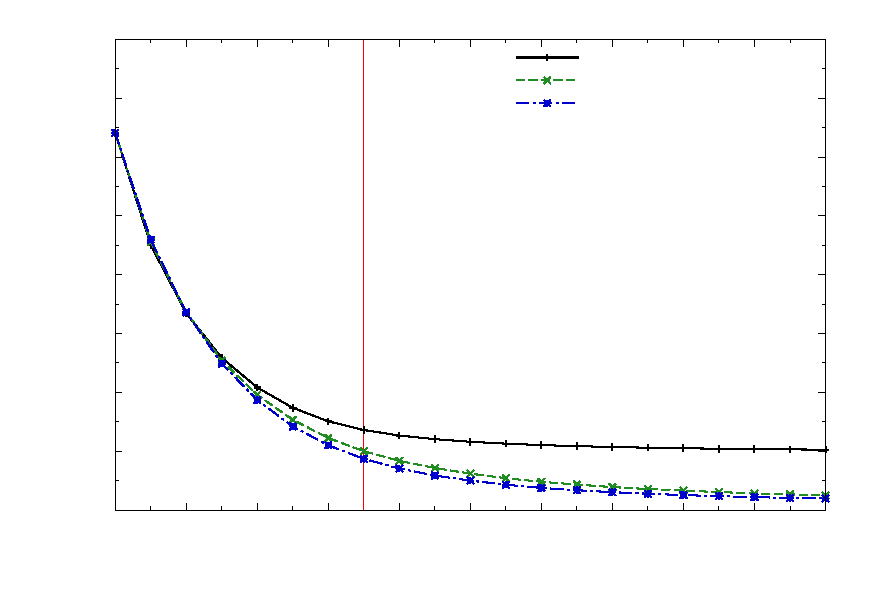
\includegraphics{plot_wind_bess_nmae}}%
    \gplfronttext
  \end{picture}%
\endgroup

		}
	\end{figure}
	
	{\scriptsize \textit{Normalised mean absolute error (NMAE) is calculated as the absolute difference between wind power forecast and actual output divided by the nominal capacity of the wind farm}
	\par
	}

\end{frame}

%%=========================================================================================%%
\begin{frame}
	\frametitle{Virtual trials}
	\framesubtitle{Snowtown wind farm coupled with a utility-scale battery}

	\begin{figure}[!h]
		\centering
    		\label{fig:disp_wind_bess}
		\scalebox{0.75}{
			% GNUPLOT: LaTeX picture with Postscript
\begingroup
  \makeatletter
  \providecommand\color[2][]{%
    \GenericError{(gnuplot) \space\space\space\@spaces}{%
      Package color not loaded in conjunction with
      terminal option `colourtext'%
    }{See the gnuplot documentation for explanation.%
    }{Either use 'blacktext' in gnuplot or load the package
      color.sty in LaTeX.}%
    \renewcommand\color[2][]{}%
  }%
  \providecommand\includegraphics[2][]{%
    \GenericError{(gnuplot) \space\space\space\@spaces}{%
      Package graphicx or graphics not loaded%
    }{See the gnuplot documentation for explanation.%
    }{The gnuplot epslatex terminal needs graphicx.sty or graphics.sty.}%
    \renewcommand\includegraphics[2][]{}%
  }%
  \providecommand\rotatebox[2]{#2}%
  \@ifundefined{ifGPcolor}{%
    \newif\ifGPcolor
    \GPcolorfalse
  }{}%
  \@ifundefined{ifGPblacktext}{%
    \newif\ifGPblacktext
    \GPblacktexttrue
  }{}%
  % define a \g@addto@macro without @ in the name:
  \let\gplgaddtomacro\g@addto@macro
  % define empty templates for all commands taking text:
  \gdef\gplbacktext{}%
  \gdef\gplfronttext{}%
  \makeatother
  \ifGPblacktext
    % no textcolor at all
    \def\colorrgb#1{}%
    \def\colorgray#1{}%
  \else
    % gray or color?
    \ifGPcolor
      \def\colorrgb#1{\color[rgb]{#1}}%
      \def\colorgray#1{\color[gray]{#1}}%
      \expandafter\def\csname LTw\endcsname{\color{white}}%
      \expandafter\def\csname LTb\endcsname{\color{black}}%
      \expandafter\def\csname LTa\endcsname{\color{black}}%
      \expandafter\def\csname LT0\endcsname{\color[rgb]{1,0,0}}%
      \expandafter\def\csname LT1\endcsname{\color[rgb]{0,1,0}}%
      \expandafter\def\csname LT2\endcsname{\color[rgb]{0,0,1}}%
      \expandafter\def\csname LT3\endcsname{\color[rgb]{1,0,1}}%
      \expandafter\def\csname LT4\endcsname{\color[rgb]{0,1,1}}%
      \expandafter\def\csname LT5\endcsname{\color[rgb]{1,1,0}}%
      \expandafter\def\csname LT6\endcsname{\color[rgb]{0,0,0}}%
      \expandafter\def\csname LT7\endcsname{\color[rgb]{1,0.3,0}}%
      \expandafter\def\csname LT8\endcsname{\color[rgb]{0.5,0.5,0.5}}%
    \else
      % gray
      \def\colorrgb#1{\color{black}}%
      \def\colorgray#1{\color[gray]{#1}}%
      \expandafter\def\csname LTw\endcsname{\color{white}}%
      \expandafter\def\csname LTb\endcsname{\color{black}}%
      \expandafter\def\csname LTa\endcsname{\color{black}}%
      \expandafter\def\csname LT0\endcsname{\color{black}}%
      \expandafter\def\csname LT1\endcsname{\color{black}}%
      \expandafter\def\csname LT2\endcsname{\color{black}}%
      \expandafter\def\csname LT3\endcsname{\color{black}}%
      \expandafter\def\csname LT4\endcsname{\color{black}}%
      \expandafter\def\csname LT5\endcsname{\color{black}}%
      \expandafter\def\csname LT6\endcsname{\color{black}}%
      \expandafter\def\csname LT7\endcsname{\color{black}}%
      \expandafter\def\csname LT8\endcsname{\color{black}}%
    \fi
  \fi
    \setlength{\unitlength}{0.0500bp}%
    \ifx\gptboxheight\undefined%
      \newlength{\gptboxheight}%
      \newlength{\gptboxwidth}%
      \newsavebox{\gptboxtext}%
    \fi%
    \setlength{\fboxrule}{0.5pt}%
    \setlength{\fboxsep}{1pt}%
\begin{picture}(8162.00,5442.00)%
    \gplgaddtomacro\gplbacktext{%
      \csname LTb\endcsname%%
      \put(946,704){\makebox(0,0)[r]{\strut{}0.0}}%
      \put(946,1080){\makebox(0,0)[r]{\strut{}5.0}}%
      \put(946,1457){\makebox(0,0)[r]{\strut{}10.0}}%
      \put(946,1833){\makebox(0,0)[r]{\strut{}15.0}}%
      \put(946,2210){\makebox(0,0)[r]{\strut{}20.0}}%
      \put(946,2586){\makebox(0,0)[r]{\strut{}25.0}}%
      \put(946,2963){\makebox(0,0)[r]{\strut{}30.0}}%
      \put(946,3339){\makebox(0,0)[r]{\strut{}35.0}}%
      \put(946,3715){\makebox(0,0)[r]{\strut{}40.0}}%
      \put(946,4092){\makebox(0,0)[r]{\strut{}45.0}}%
      \put(946,4468){\makebox(0,0)[r]{\strut{}50.0}}%
      \put(946,4845){\makebox(0,0)[r]{\strut{}55.0}}%
      \put(946,5221){\makebox(0,0)[r]{\strut{}60.0}}%
      \put(1078,484){\makebox(0,0){\strut{}0.00}}%
      \put(1646,484){\makebox(0,0){\strut{}0.10}}%
      \put(2213,484){\makebox(0,0){\strut{}0.20}}%
      \put(2781,484){\makebox(0,0){\strut{}0.30}}%
      \put(3348,484){\makebox(0,0){\strut{}0.40}}%
      \put(3916,484){\makebox(0,0){\strut{}0.50}}%
      \put(4483,484){\makebox(0,0){\strut{}0.60}}%
      \put(5051,484){\makebox(0,0){\strut{}0.70}}%
      \put(5618,484){\makebox(0,0){\strut{}0.80}}%
      \put(6185,484){\makebox(0,0){\strut{}0.90}}%
      \put(6753,484){\makebox(0,0){\strut{}1.00}}%
      \put(6885,704){\makebox(0,0)[l]{\strut{}0.0}}%
      \put(6885,1156){\makebox(0,0)[l]{\strut{}2.0}}%
      \put(6885,1607){\makebox(0,0)[l]{\strut{}4.0}}%
      \put(6885,2059){\makebox(0,0)[l]{\strut{}6.0}}%
      \put(6885,2511){\makebox(0,0)[l]{\strut{}8.0}}%
      \put(6885,2963){\makebox(0,0)[l]{\strut{}10.0}}%
      \put(6885,3414){\makebox(0,0)[l]{\strut{}12.0}}%
      \put(6885,3866){\makebox(0,0)[l]{\strut{}14.0}}%
      \put(6885,4318){\makebox(0,0)[l]{\strut{}16.0}}%
      \put(6885,4769){\makebox(0,0)[l]{\strut{}18.0}}%
      \put(6885,5221){\makebox(0,0)[l]{\strut{}20.0}}%
    }%
    \gplgaddtomacro\gplfronttext{%
      \csname LTb\endcsname%%
      \put(198,2962){\rotatebox{-270}{\makebox(0,0){\strut{}\shortstack{Proportion of dispatch intervals in which\\power dispatched is less than scheduled, \%}}}}%
      \put(7809,2962){\rotatebox{-270}{\makebox(0,0){\strut{}\shortstack{Normalised mean absolute error for dispatch intervals\\in which power dispatched is less than scheduled, \%}}}}%
      \put(3915,154){\makebox(0,0){\strut{}Battery power rating/ energy capacity, p.u.}}%
    }%
    \gplbacktext
    \put(0,0){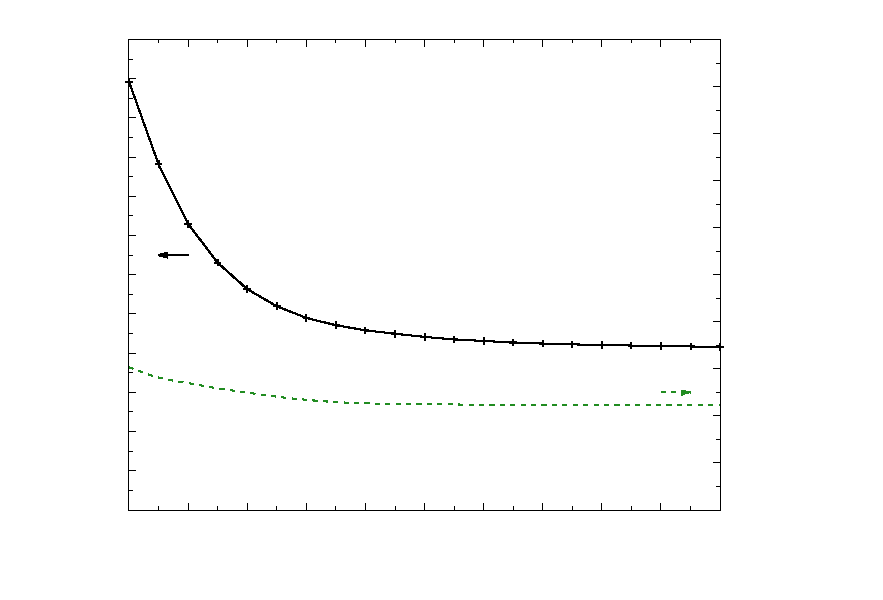
\includegraphics{plot_wind_bess_nmae_deficit}}%
    \gplfronttext
  \end{picture}%
\endgroup

		}
	\end{figure}

\end{frame}

%%=========================================================================================%%
\begin{frame}
	\frametitle{Virtual trials}
	\framesubtitle{Snowtown wind farm coupled with a utility-scale battery}

	\begin{figure}[!h]
		\centering
    		\label{fig:disp_wind_bess}
		\scalebox{0.75}{
			% GNUPLOT: LaTeX picture with Postscript
\begingroup
  \makeatletter
  \providecommand\color[2][]{%
    \GenericError{(gnuplot) \space\space\space\@spaces}{%
      Package color not loaded in conjunction with
      terminal option `colourtext'%
    }{See the gnuplot documentation for explanation.%
    }{Either use 'blacktext' in gnuplot or load the package
      color.sty in LaTeX.}%
    \renewcommand\color[2][]{}%
  }%
  \providecommand\includegraphics[2][]{%
    \GenericError{(gnuplot) \space\space\space\@spaces}{%
      Package graphicx or graphics not loaded%
    }{See the gnuplot documentation for explanation.%
    }{The gnuplot epslatex terminal needs graphicx.sty or graphics.sty.}%
    \renewcommand\includegraphics[2][]{}%
  }%
  \providecommand\rotatebox[2]{#2}%
  \@ifundefined{ifGPcolor}{%
    \newif\ifGPcolor
    \GPcolorfalse
  }{}%
  \@ifundefined{ifGPblacktext}{%
    \newif\ifGPblacktext
    \GPblacktexttrue
  }{}%
  % define a \g@addto@macro without @ in the name:
  \let\gplgaddtomacro\g@addto@macro
  % define empty templates for all commands taking text:
  \gdef\gplbacktext{}%
  \gdef\gplfronttext{}%
  \makeatother
  \ifGPblacktext
    % no textcolor at all
    \def\colorrgb#1{}%
    \def\colorgray#1{}%
  \else
    % gray or color?
    \ifGPcolor
      \def\colorrgb#1{\color[rgb]{#1}}%
      \def\colorgray#1{\color[gray]{#1}}%
      \expandafter\def\csname LTw\endcsname{\color{white}}%
      \expandafter\def\csname LTb\endcsname{\color{black}}%
      \expandafter\def\csname LTa\endcsname{\color{black}}%
      \expandafter\def\csname LT0\endcsname{\color[rgb]{1,0,0}}%
      \expandafter\def\csname LT1\endcsname{\color[rgb]{0,1,0}}%
      \expandafter\def\csname LT2\endcsname{\color[rgb]{0,0,1}}%
      \expandafter\def\csname LT3\endcsname{\color[rgb]{1,0,1}}%
      \expandafter\def\csname LT4\endcsname{\color[rgb]{0,1,1}}%
      \expandafter\def\csname LT5\endcsname{\color[rgb]{1,1,0}}%
      \expandafter\def\csname LT6\endcsname{\color[rgb]{0,0,0}}%
      \expandafter\def\csname LT7\endcsname{\color[rgb]{1,0.3,0}}%
      \expandafter\def\csname LT8\endcsname{\color[rgb]{0.5,0.5,0.5}}%
    \else
      % gray
      \def\colorrgb#1{\color{black}}%
      \def\colorgray#1{\color[gray]{#1}}%
      \expandafter\def\csname LTw\endcsname{\color{white}}%
      \expandafter\def\csname LTb\endcsname{\color{black}}%
      \expandafter\def\csname LTa\endcsname{\color{black}}%
      \expandafter\def\csname LT0\endcsname{\color{black}}%
      \expandafter\def\csname LT1\endcsname{\color{black}}%
      \expandafter\def\csname LT2\endcsname{\color{black}}%
      \expandafter\def\csname LT3\endcsname{\color{black}}%
      \expandafter\def\csname LT4\endcsname{\color{black}}%
      \expandafter\def\csname LT5\endcsname{\color{black}}%
      \expandafter\def\csname LT6\endcsname{\color{black}}%
      \expandafter\def\csname LT7\endcsname{\color{black}}%
      \expandafter\def\csname LT8\endcsname{\color{black}}%
    \fi
  \fi
    \setlength{\unitlength}{0.0500bp}%
    \ifx\gptboxheight\undefined%
      \newlength{\gptboxheight}%
      \newlength{\gptboxwidth}%
      \newsavebox{\gptboxtext}%
    \fi%
    \setlength{\fboxrule}{0.5pt}%
    \setlength{\fboxsep}{1pt}%
\begin{picture}(8162.00,5442.00)%
    \gplgaddtomacro\gplbacktext{%
      \csname LTb\endcsname%%
      \put(946,704){\makebox(0,0)[r]{\strut{}0.0}}%
      \put(946,1156){\makebox(0,0)[r]{\strut{}1.0}}%
      \put(946,1607){\makebox(0,0)[r]{\strut{}2.0}}%
      \put(946,2059){\makebox(0,0)[r]{\strut{}3.0}}%
      \put(946,2511){\makebox(0,0)[r]{\strut{}4.0}}%
      \put(946,2963){\makebox(0,0)[r]{\strut{}5.0}}%
      \put(946,3414){\makebox(0,0)[r]{\strut{}6.0}}%
      \put(946,3866){\makebox(0,0)[r]{\strut{}7.0}}%
      \put(946,4318){\makebox(0,0)[r]{\strut{}8.0}}%
      \put(946,4769){\makebox(0,0)[r]{\strut{}9.0}}%
      \put(946,5221){\makebox(0,0)[r]{\strut{}10.0}}%
      \put(1078,484){\makebox(0,0){\strut{}0.00}}%
      \put(1747,484){\makebox(0,0){\strut{}0.10}}%
      \put(2415,484){\makebox(0,0){\strut{}0.20}}%
      \put(3084,484){\makebox(0,0){\strut{}0.30}}%
      \put(3753,484){\makebox(0,0){\strut{}0.40}}%
      \put(4422,484){\makebox(0,0){\strut{}0.50}}%
      \put(5090,484){\makebox(0,0){\strut{}0.60}}%
      \put(5759,484){\makebox(0,0){\strut{}0.70}}%
      \put(6428,484){\makebox(0,0){\strut{}0.80}}%
      \put(7096,484){\makebox(0,0){\strut{}0.90}}%
      \put(7765,484){\makebox(0,0){\strut{}1.00}}%
      \put(3485,2963){\makebox(0,0)[l]{\strut{}\small Capacity factor = 0.349}}%
    }%
    \gplgaddtomacro\gplfronttext{%
      \csname LTb\endcsname%%
      \put(198,2962){\rotatebox{-270}{\makebox(0,0){\strut{}Normalised mean absolute error, \%}}}%
      \put(4421,154){\makebox(0,0){\strut{}Battery power rating/ energy capacity, p.u.}}%
      \csname LTb\endcsname%%
      \put(5389,5048){\makebox(0,0)[l]{\strut{}\small 30-minute control horizon}}%
      \csname LTb\endcsname%%
      \put(5389,4828){\makebox(0,0)[l]{\strut{}\small 60-minute control horizon}}%
    }%
    \gplbacktext
    \put(0,0){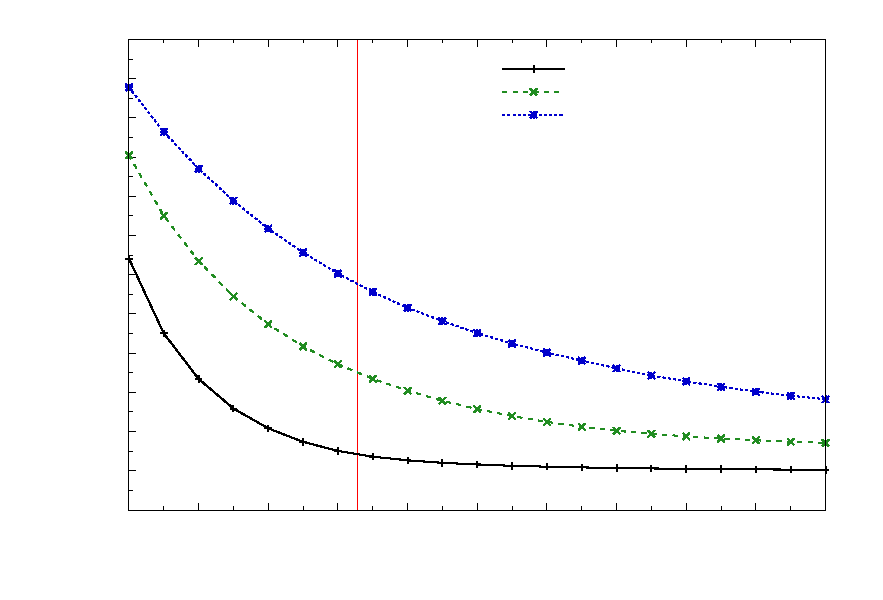
\includegraphics{plot_wind_bess_nmae_hrzn}}%
    \gplfronttext
  \end{picture}%
\endgroup

		}
	\end{figure}

\end{frame}


%%=========================================================================================%%
\begin{frame}
	\frametitle{Direction of future research}
	\framesubtitle{}

	
\end{frame}

%%=========================================================================================%%
\end{document}

%%=========================================================================================%%
%%=========================================================================================%%
\begin{frame}
	\frametitle{<frame title>}
	\subframetitle{<subframe title>}

	<introductory statement>
	\begin{itemize}
		\item  <first item>
		\item  <more items>
	\end{itemize}
	
	\begin{figure}[!h]
	\centering
    	\label{fig:<label>}
	\scalebox{0.80}{
		\includegraphics{<file.pdf>}
		\input{<file>}
	}
	\end{figure}
	

\note[item]{
<notes>
}
\end{frame}

%%=========================================================================================%%


